\section{Diseño de la Plataforma Base}

\subsection{Dimensionamiento de la Plataforma Base}

Una vez seleccionada la canastilla plástica como contenedor definitivo del kit, se procedió a realizar un levantamiento dimensional completo mediante mediciones directas del producto adquirido. Estas mediciones permitieron establecer las restricciones geométricas que determinarían las dimensiones finales de la plataforma base.

Con el objetivo de maximizar el aprovechamiento del espacio disponible dentro del contenedor, se desarrolló un modelo digital tridimensional de la canastilla que permitió visualizar las restricciones espaciales y planificar la distribución óptima de componentes.

Como se observa en la Figura \ref{fig:carcasa}, la canastilla presenta las siguientes dimensiones:

\begin{itemize}
    \item \textbf{Dimensiones externas}: 600 mm × 400 mm
    \item \textbf{Dimensiones internas útiles}: 566 mm × 366 mm
    \item \textbf{Espesor de pared}: 17 mm (calculado a partir de la diferencia entre dimensiones externas e internas)
\end{itemize}


Considerando las dimensiones internas de la canastilla y la necesidad de dejar holguras mínimas para facilitar el montaje y desmontaje de la plataforma, se establecieron las siguientes dimensiones preliminares para la plataforma base:

\begin{itemize}
    \item \textbf{Ancho de la plataforma}: 365 mm
    \item \textbf{Largo de la plataforma}: 560 mm
\end{itemize}

Estas dimensiones proporcionan:

\begin{itemize}
    \item Holgura lateral: $\frac{566 - 560}{2} = 3$ mm por cada lado en el eje longitudinal
    \item Holgura frontal: $\frac{366 - 365}{2} = 0.5$ mm por cada lado en el eje transversal
\end{itemize}

La selección de estas dimensiones se fundamenta en los siguientes criterios de diseño:

\begin{enumerate}
    \item \textbf{Maximización del espacio útil}: Las dimensiones propuestas aprovechan el 99.3\% del espacio interno disponible en la canastilla (560 mm × 365 mm de 566 mm × 366 mm)
    
    \item \textbf{Tolerancias de ensamblaje}: Las holguras mínimas (0.5 mm - 3 mm) permiten compensar tolerancias dimensionales tanto de la canastilla comercial como de la plataforma a fabricar, facilitando operaciones de montaje y desmontaje
    
    \item \textbf{Compatibilidad con espacio de trabajo del robot}: El largo de 560 mm permite ubicar el robot en posición central con un radio de alcance efectivo de 280 mm, cumpliendo con la restricción de 28.3 cm establecida previamente
    
    \item \textbf{Distribución de zonas funcionales}: El ancho de 365 mm permite distribuir adecuadamente las zonas de recolección, depósito y electrónica a lo largo de la plataforma
\end{enumerate}

Estas dimensiones preliminares serán validadas mediante modelado 3D completo del kit, donde se verificará la disposición espacial de todos los componentes (robot, zonas de trabajo, electrónica, sistema de visión) dentro de los límites establecidos. En caso de identificarse interferencias o restricciones adicionales durante el proceso de diseño detallado, las dimensiones podrán ser ajustadas manteniendo el criterio de máximo aprovechamiento del espacio disponible.


\subsection{Primera Iteración del Diseño de la Plataforma}

\subsubsection{Concepto de Diseño Modular}

Para la primera iteración del diseño de la plataforma, se desarrolló un concepto basado en modularidad y reconfigurabilidad. El objetivo principal fue crear un sistema flexible que permitiera reposicionar las zonas de recolección y depósito según las necesidades didácticas del kit, facilitando diferentes configuraciones experimentales para los estudiantes.

El diseño inicial se fundamentó en una distribución tipo layout que buscaba ubicar los distintos componentes del kit sobre la plataforma base. La estrategia de modularidad se implementó mediante un sistema de celdas cuadradas equipadas con imanes de neodimio, los cuales permitirían el anclaje y reconfiguración de las zonas funcionales sin necesidad de herramientas.

\subsubsection{Componentes del Diseño Inicial}

El modelo 3D de la primera versión del kit comprendía los siguientes componentes, cuyas especificaciones detalladas se presentarán en las secciones correspondientes a cada elemento:

\begin{enumerate}
    \item \textbf{Plataforma base}: Superficie principal de montaje fabricada en MDF de 9 mm de espesor
    
    \item \textbf{Módulos cuadrados}: 18 unidades, cada una equipada con 4 imanes de neodimio en su interior para permitir el anclaje de componentes
    
    \item \textbf{Módulos rectangulares}: 12 unidades, cada una con 2 imanes de neodimio integrados
    
    \item \textbf{Zonas de recolección cuadradas}: 2 unidades, cada una equipada con 16 imanes de neodimio para asegurar su fijación a la plataforma
    
    \item \textbf{Zonas de depósito tipo caneca}: Dos tipos diferenciados por tamaño
    \begin{itemize}
        \item 2 canecas grandes, cada una con 7 imanes de neodimio
        \item 3 canecas pequeñas, cada una con 4 imanes de neodimio
        \item Todas las canecas equipadas con tapas de bisagra para contener objetos durante el transporte del kit
    \end{itemize}
    
    \item \textbf{Soporte de cámara}: Estructura vertical con espacio de anclaje dedicado en la plataforma
    
    \item \textbf{Base del manipulador}: Área de montaje específica para el robot PhantomX Pincher
\end{enumerate}

La Figura \ref{fig:primerDiseñoConceptualKit} presenta el ensamble completo de la plataforma con todos sus componentes integrados, donde se identifican los elementos mediante numeración:

\begin{figure}[H]
    \centering
    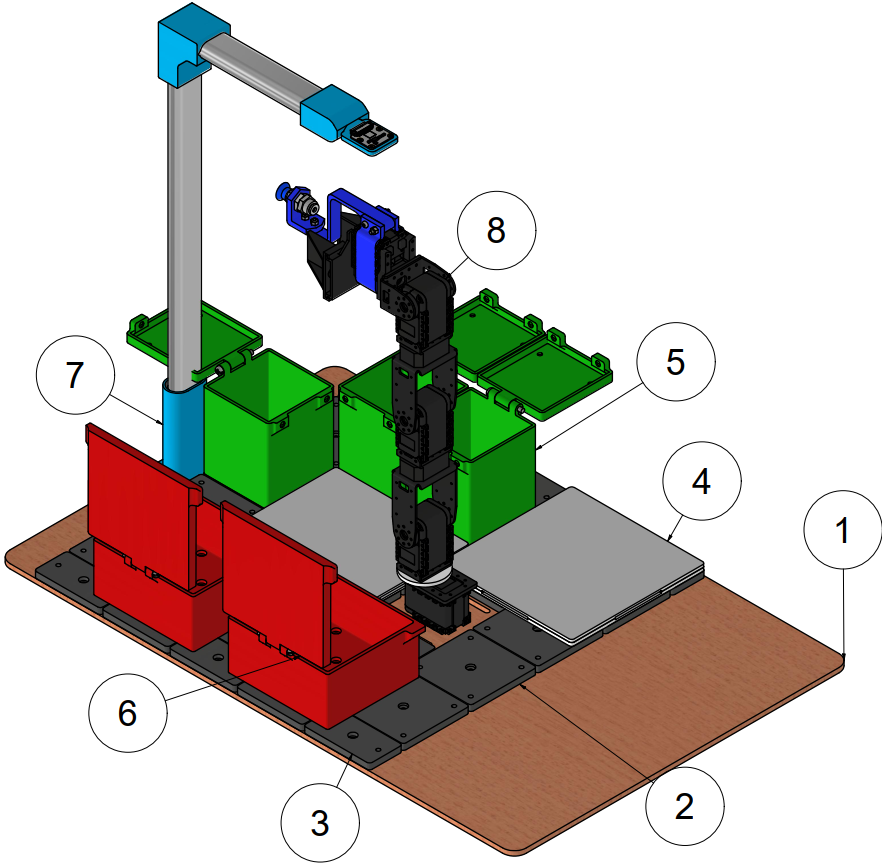
\includegraphics[width=0.9\textwidth]{06disenoConceptual/img/plataforma/ensambleKitObsoleto.png}
    \caption{Primera iteración del diseño conceptual del kit. (1) Plataforma base, (2) Módulo cuadrado, (3) Módulo rectangular, (4) Zona de recolección cuadrada, (5) Caneca pequeña, (6) Caneca grande, (7) Soporte de cámara, (8) Brazo robótico o manipulador}
    \label{fig:primerDiseñoConceptualKit}
\end{figure}

\subsubsection{Desarrollo del Layout de la Plataforma}

El proceso de diseño del layout se desarrolló en dos etapas iterativas:

\paragraph{Layout Inicial - Definición del Área de Trabajo}

El primer layout (Figura \ref{fig:layout1O}) se basó en la restricción cinemática fundamental del manipulador: su alcance efectivo de 283 mm. Se inscribió un cuadrado dentro del círculo formado por dicho alcance, estableciendo así el área de trabajo primaria donde el robot podría operar con máxima libertad de movimiento.

\begin{figure}[H]
    \centering
    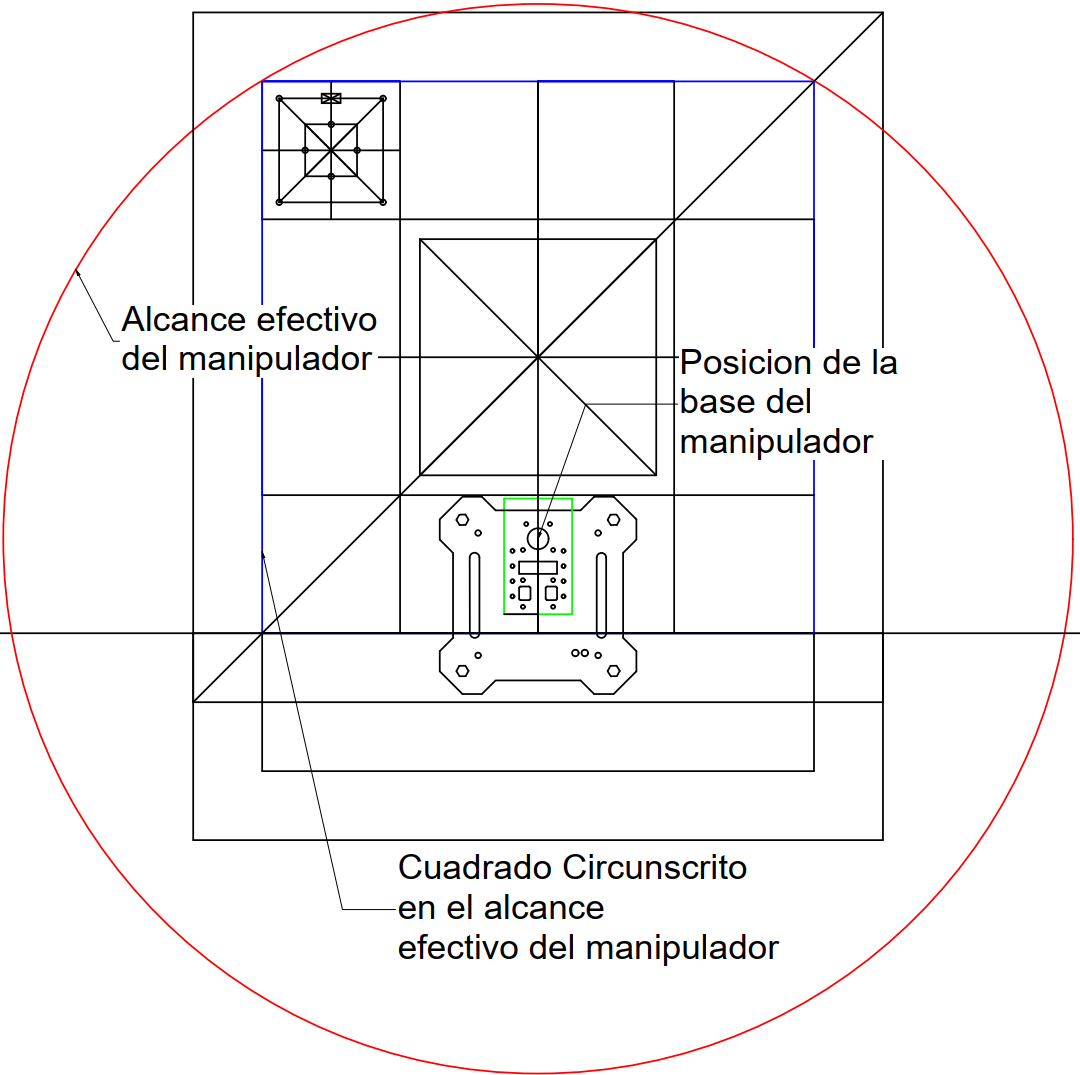
\includegraphics[width=0.7\textwidth]{06disenoConceptual/img/plataforma/layout1Obsoleto.png}
    \caption{Layout inicial de la plataforma mostrando el cuadrado circunscrito en el área de alcance efectivo del manipulador (radio de 283 mm). Se indica la posición central de la base del manipulador.}
    \label{fig:layout1O}
\end{figure}

\paragraph{Layout Refinado - Sistema de Cuadrícula Modular}

A partir del cuadrado de trabajo definido, se desarrolló un sistema de cuadrícula que sirvió como base dimensional para los módulos cuadrados y rectangulares. En esta segunda iteración del layout (Figura \ref{fig:layout2Obsoleto}), se incorporaron elementos adicionales como:

\begin{itemize}
    \item Ubicación del soporte de cámara en posición superior central
    \item Sistema de anclaje mediante orificios roscados para módulos cuadrados
    \item Sistema de anclaje para módulos rectangulares
    \item Puntos de fijación para canecas de depósito
    \item Zona de montaje de la base del manipulador
\end{itemize}

\begin{figure}[H]
    \centering
    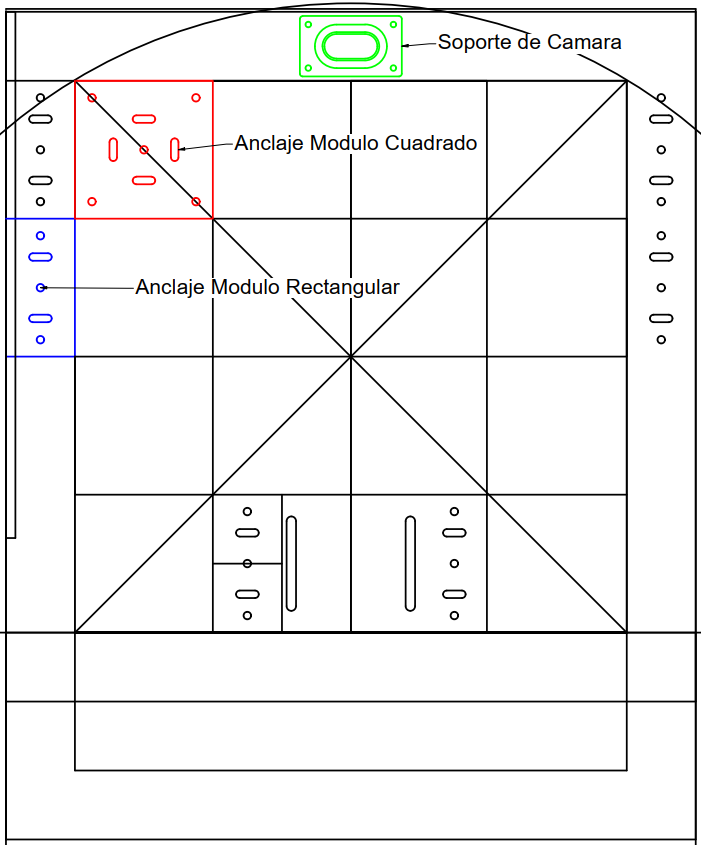
\includegraphics[width=0.7\textwidth]{06disenoConceptual/img/plataforma/layout2obsoleto.png}
    \caption{Layout refinado de la plataforma mostrando el sistema de cuadrícula modular. Se identifican los puntos de anclaje para módulos cuadrados (color rojo) y módulos rectangulares (color azul), así como la ubicación del soporte de cámara en la zona superior.}
    \label{fig:layout2Obsoleto}
\end{figure}


Finalmente se repite el patrón en la cuadricula y se obtiene el modelo 3D de la plataforma inicial que se ve en la figura \ref{fig:plataformaBaseV1.0}

\begin{figure}[H]
    \centering
    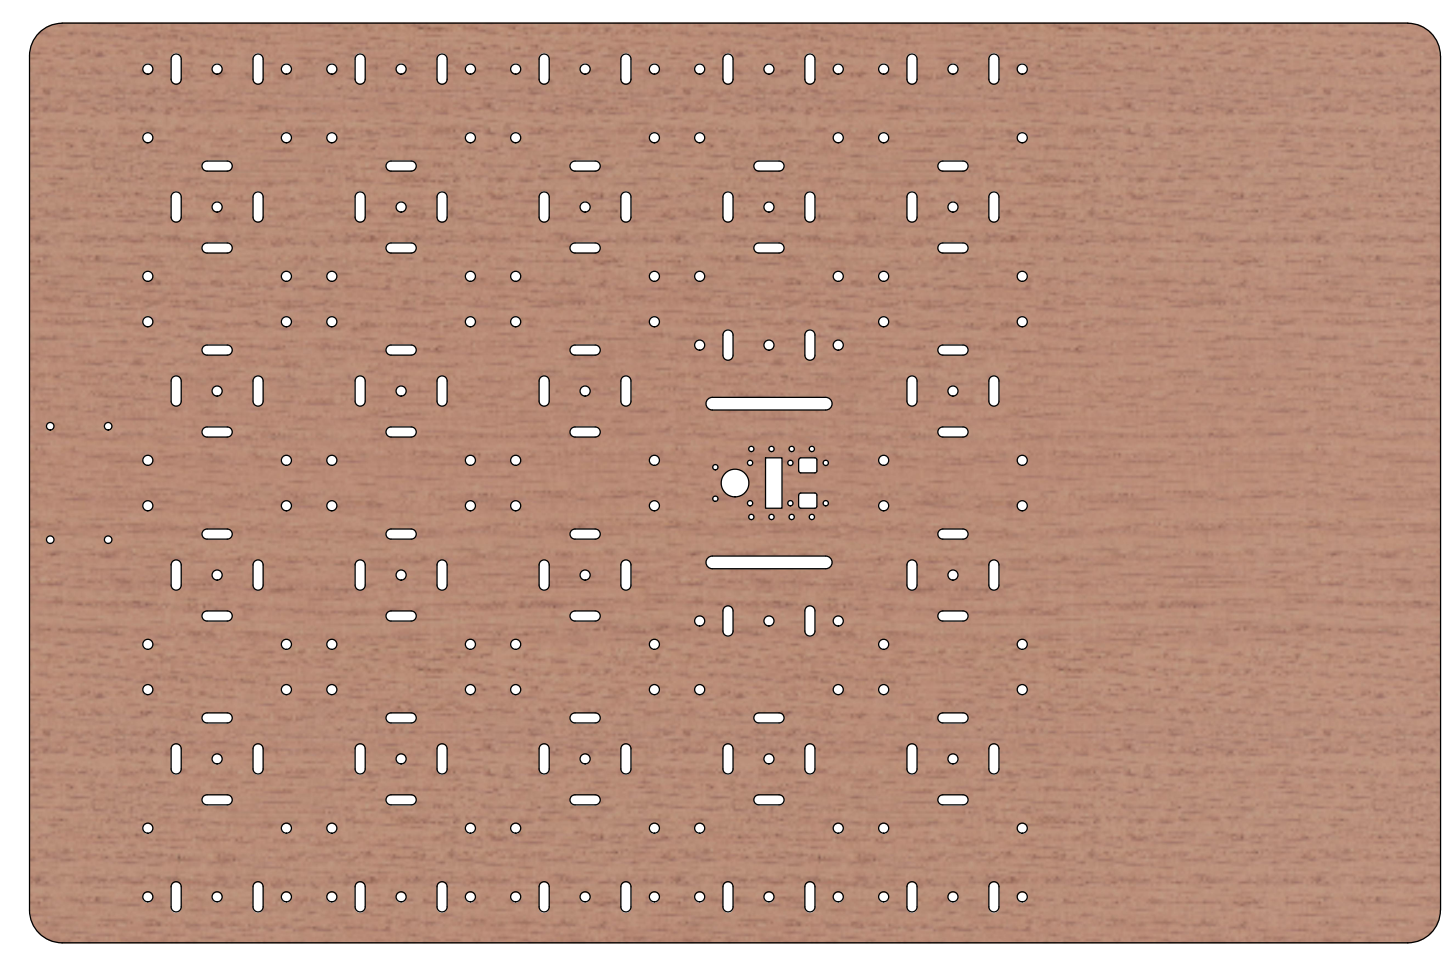
\includegraphics[width=0.7\textwidth]{06disenoConceptual/img/plataforma/plataformaBaseObsoleto.png}
    \caption{ Plataforma base version 1.}
    \label{fig:plataformaBaseV1.0}
\end{figure}

\subsubsection{Selección del Material de la Plataforma}

Para la fabricación de la plataforma base se seleccionó tablero de fibra de densidad media (MDF) de 9 mm de espesor. Esta decisión se fundamentó en un análisis comparativo de costos con materiales alternativos.

Si bien el MDF requiere un proceso de acabado superficial que incluye lijado, sellado, pintado y lacado para garantizar durabilidad y resistencia a la humedad, su relación costo-beneficio resultó significativamente superior a otras opciones consideradas.

\begin{table}[H]
\centering
\caption{Comparación de costos de materiales para la plataforma base}
\label{tab:costos_plataforma}
\begin{tabular}{|l|r|r|}
\hline
\textbf{Material} & \textbf{Costo por unidad} & \textbf{Relación de costo} \\
\hline
MDF 9 mm + corte láser & \$25,000 COP & 1.0× (referencia) \\
Acrílico 9 mm + corte láser & \$200,000 COP & 8.0× \\
\hline
\end{tabular}
\end{table}

El acrílico, a pesar de ofrecer ventajas en términos de resistencia a la humedad y acabado superficial, presentó un costo 8 veces superior al MDF. Considerando que se deben fabricar 7 plataformas (una por cada kit), la diferencia total ascendería a \$1,225,000 COP (\$175,000 en MDF vs \$1,400,000 en acrílico), lo cual excede significativamente el presupuesto disponible por kit.

\subsubsection{Problemas Identificados y Rechazo del Diseño}

A pesar del esfuerzo de diseño invertido, esta primera iteración fue rechazada debido a múltiples deficiencias críticas identificadas durante el proceso de evaluación:

\begin{enumerate}
    \item \textbf{Complejidad excesiva del sistema}: El diseño presentaba un número excesivo de partes móviles e interdependientes, lo cual comprometía la robustez y facilidad de uso del kit. El sistema de 178 imanes de neodimio (distribuidos en módulos, zonas de recolección y canecas) representaba:
    \begin{itemize}
        \item Costo elevado en componentes de fijación
        \item Dificultad en el ensamblaje y mantenimiento
        \item Complejidad innecesaria para los objetivos didácticos del kit
    \end{itemize}
    
    \item \textbf{Dimensionamiento inadecuado de la plataforma}: Las dimensiones de ancho y largo de la plataforma no consideraron las tolerancias de fabricación de la canastilla plástica comercial. Las paredes del contenedor pueden presentar cierta flexión debido a su proceso de moldeo por inyección, lo que dificultaba la extracción e inserción de la plataforma. Las holguras previstas (0.5 mm - 3 mm) resultaron insuficientes en la práctica.
    
    \item \textbf{Error fundamental en el análisis cinemático}: Se cometió un error crítico en el proceso de diseño al no considerar adecuadamente las limitaciones cinemáticas del manipulador. El PhantomX Pincher, al poseer únicamente 4 grados de libertad (DOF), presenta restricciones significativas en su capacidad de orientación del efector final. El uso de una cuadrícula regular como layout asumía implícitamente que el robot podría alcanzar cualquier posición con cualquier orientación, lo cual es cinemáticamente incorrecto para un manipulador de 4 DOF.
    
    Esta limitación implicaba que ciertas celdas de la cuadrícula resultarían inaccesibles o accesibles solo con orientaciones específicas del efector final, comprometiendo la funcionalidad del sistema modular propuesto.
    
    \item \textbf{Ausencia de sistema de manipulación}: No se contempló un método ergonómico y práctico para extraer e insertar la plataforma del contenedor. La ausencia de asas, agarraderas o sistemas de sujeción dificultaba el manejo del kit, especialmente considerando el peso combinado de la plataforma, el robot y los componentes electrónicos.
    
    \item \textbf{Omisión del subsistema electrónico}: El diseño no incluyó una ubicación dedicada para los componentes electrónicos del sistema (controlador, fuente de alimentación, cableado). Esta omisión representaba un problema fundamental, ya que la electrónica constituye un elemento esencial del kit que requiere espacio protegido, ventilación adecuada y accesibilidad para mantenimiento.
\end{enumerate}

\subsubsection{Lecciones Aprendidas}

El proceso de diseño y evaluación crítica de esta primera iteración proporcionó valiosas lecciones que orientaron el desarrollo de versiones subsecuentes:

\begin{itemize}
    \item La modularidad excesiva puede comprometer la funcionalidad y aumentar innecesariamente la complejidad
    \item Las restricciones cinemáticas del manipulador deben ser el punto de partida fundamental del diseño, no una consideración posterior
    \item Las tolerancias de fabricación de componentes comerciales deben verificarse mediante prototipos físicos
    \item El diseño debe considerar todos los subsistemas desde las etapas iniciales (mecánico, electrónico, interfaz de usuario)
    \item La simplicidad y robustez son preferibles a la versatilidad cuando esta última compromete la usabilidad
\end{itemize}

Estas observaciones fundamentaron el desarrollo de una segunda iteración del diseño, la cual se presenta en la siguiente sección.

\subsection{Segunda Iteración del Diseño de la Plataforma}

\subsubsection{Principios de Diseño Revisados}

La segunda iteración del diseño incorporó las lecciones aprendidas del primer prototipo, adoptando un enfoque fundamentalmente diferente basado en los siguientes principios rectores:

\begin{enumerate}
    \item \textbf{Eliminación de la modularidad excesiva}: Las zonas de recolección y depósito se diseñaron como elementos fijos, eliminando el sistema de imanes y módulos intercambiables que añadían complejidad innecesaria
    
    \item \textbf{Simplificación del sistema de clasificación}: Se redujo a una única zona de recolección circular y cuatro zonas de depósito de igual área, simplificando la operación y el software de control
    
    \item \textbf{Integración del subsistema electrónico}: Se incorporó desde el inicio un área dedicada para la Raspberry Pi y una zona flexible para componentes electrónicos adicionales
    
    \item \textbf{Consideración de restricciones cinemáticas}: El posicionamiento de las zonas de trabajo se basó en el análisis del alcance efectivo y las limitaciones de 4 DOF del manipulador
    
    \item \textbf{Mejora de la ergonomía}: Se añadieron manijas para facilitar la manipulación de la plataforma
    
    \item \textbf{Estabilidad y nivelación}: Se incorporaron patas niveladoras en las esquinas y patas de soporte centrales para garantizar estabilidad
    
    \item \textbf{Gestión de cableado}: Se diseñaron canaletas específicas para el paso ordenado de cables
    
    \item \textbf{Sistema de vacío}: Se integró el montaje de la bomba de vacío requerida para el nuevo sistema de sujeción
\end{enumerate}

\subsubsection{Arquitectura de Diseño en Dos Niveles}

A diferencia del diseño anterior, esta iteración requirió considerar la plataforma como un sistema de dos niveles funcionales:

\paragraph{Nivel Superior}
Comprende todos los componentes operativos montados sobre la superficie de la plataforma: zonas de trabajo (recolección y depósito), manipulador, sistema de visión, electrónica de control y sistema de vacío.

\paragraph{Nivel Inferior}
Incluye los elementos estructurales y de servicio ubicados en la cara inferior de la plataforma: sistema de cableado, canaletas, tornillería de fijación, patas niveladoras y estructuras de soporte.

Esta arquitectura de dos niveles permite una separación clara entre funcionalidades operativas y de soporte, facilitando el mantenimiento y modificaciones futuras.

\subsubsection{Análisis de Layouts}

El diseño se desarrolló mediante tres layouts complementarios que abordan diferentes aspectos del sistema:

\paragraph{Layout 1: Análisis Cinemático de Zonas de Depósito}

El primer layout (Figura \ref{fig:layout1}) se centra en la validación cinemática de la ubicación de las zonas de depósito. Este análisis demuestra que todas las zonas de depósito se encuentran dentro del alcance efectivo del robot (círculo rojo con radio de 283 mm).

\begin{figure}[H]
    \centering
    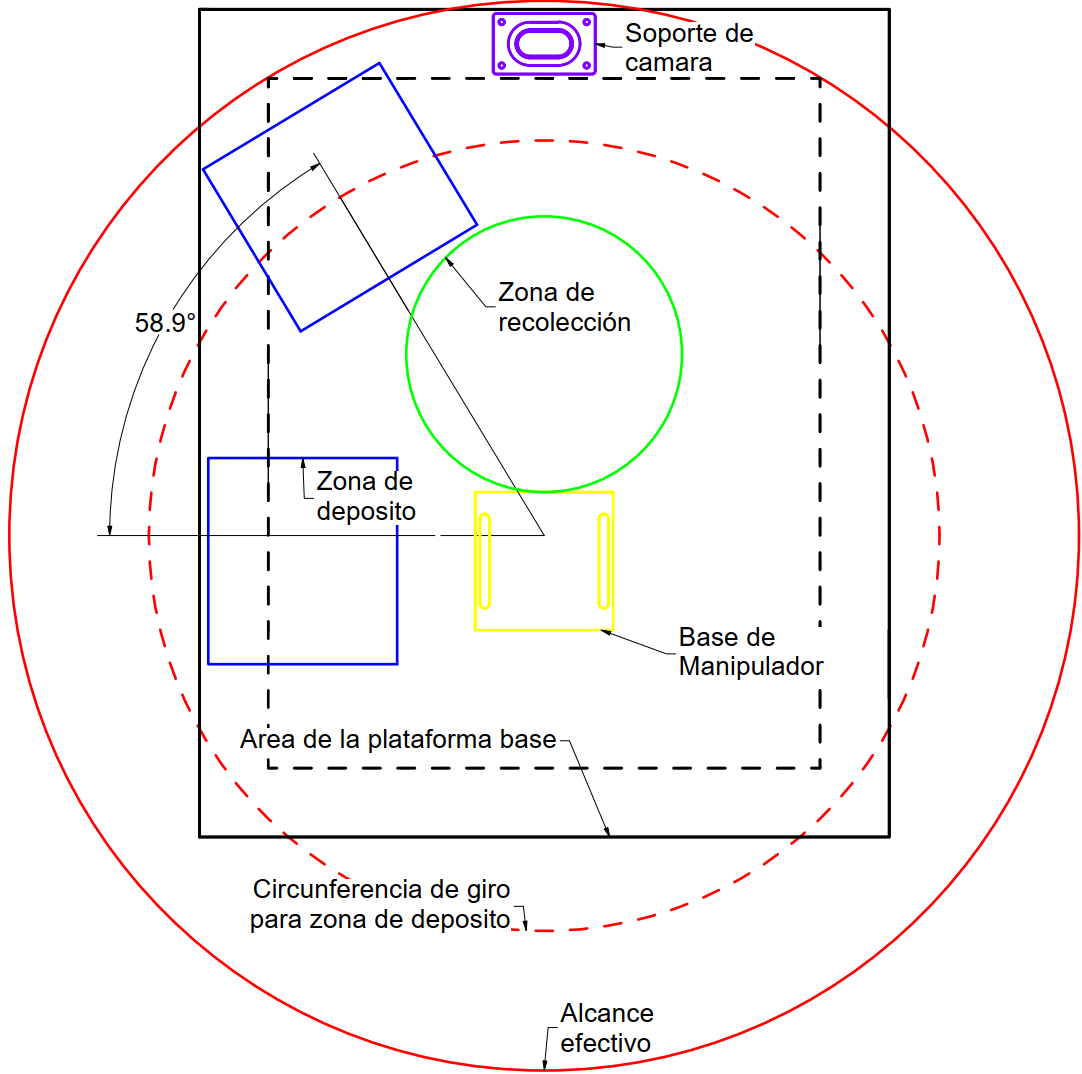
\includegraphics[width=0.75\textwidth]{06disenoConceptual/img/plataforma/layout1.png}
    \caption{Layout 1 - Análisis cinemático de accesibilidad. Se muestra cómo las cuatro zonas de depósito (azul) están contenidas dentro del alcance efectivo del manipulador (círculo rojo). El ángulo de 58.9° indica la rotación angular de las zonas de depósito alrededor del eje de la primera articulación del robot, garantizando accesibilidad desde cualquier configuración. La zona de recolección (verde) se ubica en posición central. Se indica también la circunferencia de giro (línea punteada roja) que delimita el área de trabajo óptima.}
    \label{fig:layout1}
\end{figure}

La estrategia de posicionamiento se basó en la rotación de las zonas de depósito alrededor del eje de la primera articulación (base) del robot. Como se observa en la figura, dos de las zonas de depósito se encuentran rotadas 58.9° con respecto al eje longitudinal de la plataforma. Esta disposición angular garantiza que el manipulador, con sus 4 grados de libertad, pueda alcanzar todas las zonas de depósito mediante rotación de su base y movimientos coordinados de sus eslabones, sin requerir orientaciones imposibles del efector final.

\paragraph{Layout 2: Distribución de Componentes en Nivel Superior}

El segundo layout (Figura \ref{fig:layout2}) presenta la distribución completa de componentes en el nivel superior de la plataforma:

\begin{figure}[H]
    \centering
    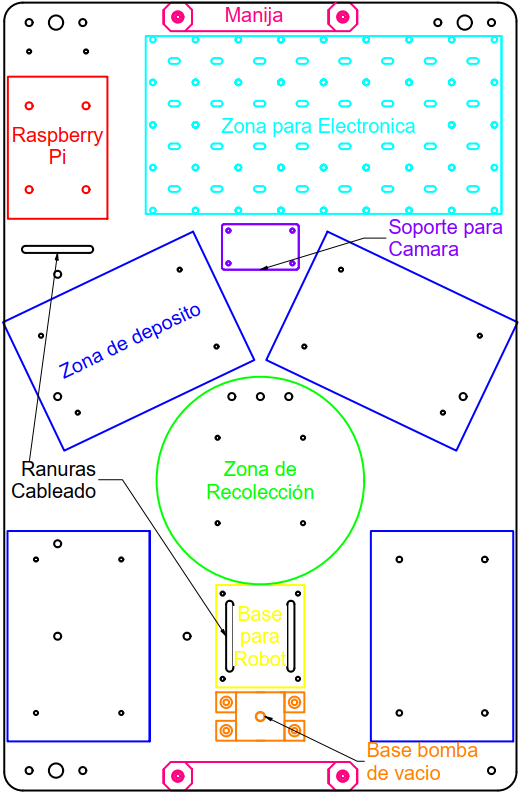
\includegraphics[width=0.75\textwidth]{06disenoConceptual/img/plataforma/layout2.png}
    \caption{Layout 2 - Vista superior de la plataforma mostrando la distribución de todos los componentes operativos. Se identifican: zona de electrónica con retícula de montaje (cian), controlador Raspberry Pi (rojo), cuatro zonas de depósito simétricas (azul), zona de recolección central (verde), base del manipulador (amarillo), soporte de cámara (morado), manijas de transporte (rosa), ranuras de cableado (negro) y base de bomba de vacío (naranja). Las dimensiones corresponden a la plataforma de 560 mm × 365 mm.}
    \label{fig:layout2}
\end{figure}

Los elementos clave identificados en este layout son:

\begin{itemize}
    \item \textbf{Zona de electrónica} (cian): Ubicada en la región posterior, más allá del área de trabajo del robot. Incorpora una retícula de montaje flexible de 30 mm × 30 mm
    \item \textbf{Controlador Raspberry Pi} (rojo): Posición dedicada con montaje específico, ubicada lateralmente para facilitar acceso a puertos
    \item \textbf{Zonas de depósito} (azul): Cuatro receptáculos idénticos distribuidos simétricamente alrededor de la zona de recolección
    \item \textbf{Zona de recolección} (verde): Área circular central donde se posicionan los objetos a clasificar
    \item \textbf{Base del manipulador} (amarillo): Montaje central con patrón de tornillería específico para el PhantomX Pincher
    \item \textbf{Soporte de cámara} (morado): Ubicado entre la zona de electrónica y el área de trabajo, proporcionando vista superior de la escena
    \item \textbf{Manijas de transporte} (rosa): Ubicadas en los bordes superior e inferior de la plataforma para facilitar manipulación
    \item \textbf{Ranuras de cableado} (negro): Aberturas estratégicas para paso de cables entre niveles
    \item \textbf{Base de bomba de vacío} (naranja): Montaje cercano a la base del robot para minimizar longitud de mangueras
\end{itemize}

\paragraph{Layout 3: Componentes del Nivel Inferior}

El tercer layout (Figura \ref{fig:layout3}) detalla los elementos estructurales y de servicio ubicados en el nivel inferior de la plataforma:

\begin{figure}[H]
    \centering
    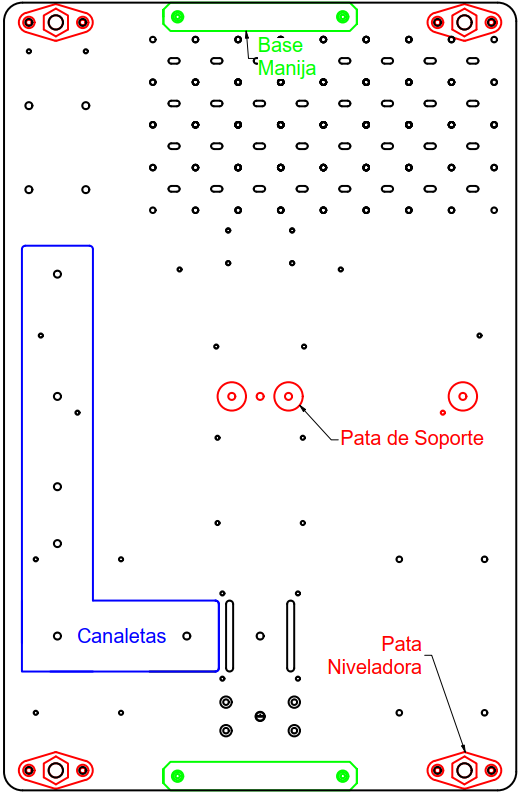
\includegraphics[width=0.75\textwidth]{06disenoConceptual/img/plataforma/layout3.png}
    \caption{Layout 3 - Vista inferior de la plataforma mostrando elementos estructurales y de servicio. Se identifican: canaletas de cableado (azul) en forma de L para gestión ordenada de cables, patas niveladoras (rojo) en las cuatro esquinas con roscas M10, patas de soporte centrales (rojo) para rigidez adicional, manijas de transporte (rosa) con tornillería M6, y base de soporte (verde) para fijación del manipulador. El patrón de agujeros permite la instalación de insertos roscados M4 para montaje de componentes.}
    \label{fig:layout3}
\end{figure}

Los componentes del nivel inferior incluyen:

\begin{itemize}
    \item \textbf{Canaletas de cableado} (azul): Configuración en forma de L que permite el ruteo ordenado de cables desde las zonas de depósito y recolección hacia la zona de electrónica
    \item \textbf{Patas niveladoras} (rojo): Ubicadas en las cuatro esquinas, con agujeros roscados M10 que alojan tornillos de nivelación ajustables
    \item \textbf{Patas de soporte centrales} (rojo): Tres puntos de apoyo adicionales que proporcionan rigidez a la plataforma y evitan flexión en la zona central
    \item \textbf{Manijas} (rosa): Montadas con tornillería M6 que atraviesa completamente la plataforma
    \item \textbf{Patrón de insertos roscados}: Distribución de posiciones para insertos de madera roscados M4 que servirán de anclaje para diversos componentes
\end{itemize}

\subsubsection{Estrategia de Posicionamiento de Zonas Funcionales}

\paragraph{Ubicación de Zonas de Depósito}

El posicionamiento de las zonas de depósito se determinó mediante el siguiente proceso:

\begin{enumerate}
    \item Se trazó el círculo de alcance efectivo del robot (radio de 283 mm) centrado en el eje de su primera articulación
    
    \item Se inscribió un cuadrado dentro de este círculo, similar al enfoque del primer diseño
    
    \item Se posicionó una zona de depósito dentro del cuadrado inscrito
    
    \item Esta zona se rotó alrededor del eje de la primera articulación del robot, generando posiciones angulares múltiples
    
    \item Se seleccionaron cuatro posiciones angulares que maximizaban la separación entre zonas mientras mantenían todas las posiciones dentro del alcance efectivo
\end{enumerate}

Esta estrategia garantiza que el manipulador puede alcanzar cualquier zona de depósito mediante una simple rotación de su base, seguida de movimientos coordinados de sus eslabones. La configuración angular de 58.9° entre zonas adyacentes permite una distribución simétrica que facilita la programación del sistema de control.

\paragraph{Zona de Recolección}

La zona de recolección se diseñó como un área circular ubicada en la región central, delimitada por:

\begin{itemize}
    \item Límite interno: Perímetro de la base del brazo robótico
    \item Límite externo: Circunferencia que conecta las zonas de depósito
\end{itemize}

Esta configuración garantiza que cualquier objeto colocado en la zona de recolección es accesible para el manipulador sin interferencias con su propia base o con las zonas de depósito.

\paragraph{Zona de Electrónica}

La zona de electrónica se ubicó estratégicamente más allá del cuadrado circunscrito en el círculo de alcance máximo del robot. Esta ubicación ofrece múltiples ventajas:

\begin{itemize}
    \item Protección física: Los componentes electrónicos quedan fuera del área de movimiento del manipulador, eliminando riesgo de colisiones
    \item Accesibilidad: Posición en el borde de la plataforma facilita conexión y desconexión de cables
    \item Ventilación: Ubicación alejada de componentes mecánicos permite mejor circulación de aire
    \item Expansibilidad: Área suficiente para añadir componentes adicionales según evolucionen los requerimientos
\end{itemize}

\subsubsection{Sistema de Retícula para Montaje Flexible}

La zona de electrónica incorpora un sistema de retícula que proporciona flexibilidad para cambios futuros en los componentes electrónicos del sistema. Esta retícula se compone de:

\paragraph{Patrón de Agujeros Circulares}
Agujeros pasantes de diámetro apropiado para alojar insertos roscados M4, distribuidos en un patrón rectangular con separación de 30 mm entre centros en ambas direcciones. Este espaciado de 30 mm fue seleccionado por:

\begin{itemize}
    \item Compatibilidad con dimensiones estándar de componentes electrónicos y mecánicos
    \item Suficiente densidad de puntos de fijación sin debilitar excesivamente la estructura de MDF
    \item Coincidencia con múltiplos de dimensiones comunes en sistemas robóticos (15 mm, 60 mm, 90 mm)
\end{itemize}

\paragraph{Ranuras de Cableado}
Ranuras oblongas integradas en el patrón de la retícula que permiten el paso de cables entre componentes montados en la superficie y el nivel inferior de la plataforma. Estas ranuras se encuentran estratégicamente ubicadas para:

\begin{itemize}
    \item Permitir conexiones entre la Raspberry Pi y periféricos
    \item Facilitar el paso de mangueras neumáticas si se requiere posicionar la bomba de vacío en la zona de electrónica (configuración alternativa)
    \item Organizar el cableado de alimentación desde fuentes externas
\end{itemize}

\paragraph{Área Dedicada del Controlador}
Además de la retícula general, se diseñó un área específica para el montaje de la Raspberry Pi, con:

\begin{itemize}
    \item Patrón de agujeros coincidente con los puntos de montaje estándar de la Raspberry Pi
    \item Ranuras adyacentes para paso de cables USB, HDMI, y alimentación
    \item Espacio perimetral para acceso a puertos laterales sin remover el controlador
\end{itemize}

La filosofía de diseño de la retícula permite que la electrónica del robot pueda ser actualizada o modificada sin necesidad de rediseñar la plataforma completa, facilitando la evolución del kit según nuevas necesidades educativas o mejoras tecnológicas.

\subsubsection{Sistemas de Fijación y Anclaje}

El diseño contempla múltiples sistemas de anclaje diferenciados según los requerimientos de carga, frecuencia de desmontaje, y tipo de componente:

\paragraph{Anclajes con Insertos Roscados de Madera M4}

Se seleccionaron insertos roscados de madera M4 como sistema de fijación principal para componentes que requieren desmontaje ocasional. Estos insertos se utilizan en:

\begin{itemize}
    \item Soporte de cámara: 4 puntos de fijación
    \item Patas niveladoras: 4 unidades en las esquinas
    \item Patas de soporte central: 3 unidades
    \item Anclaje de bomba de vacío: Configuración según modelo específico
    \item Carcasa del controlador (Raspberry Pi): 4 puntos de montaje
    \item Zonas de recolección: 4 tornillos de fijación
    \item Zonas de depósito: 4 tornillos de fijación cada una (16 tornillos totales)
    \item Base del robot: 4 tornillos de fijación
\end{itemize}

La selección de insertos roscados de madera sobre alternativas convencionales se fundamentó en:

\begin{enumerate}
    \item \textbf{Durabilidad de la rosca}: Los insertos metálicos proporcionan roscas duraderas que no se degradan con ciclos repetidos de montaje/desmontaje, a diferencia de roscas directas en MDF que se desgastan rápidamente
    
    \item \textbf{Facilidad de reemplazo}: Los componentes pueden ser removidos y reinstalados múltiples veces utilizando tornillos estándar M4, sin deterioro del punto de fijación
    
    \item \textbf{Eliminación de tuercas convencionales}: Se evita el uso de tuercas tradicionales que presentan dos problemas principales:
    \begin{itemize}
        \item Susceptibilidad a caerse o perderse durante operaciones de mantenimiento
        \item Tendencia a dañar el acabado superficial (pintura) de la plataforma debido a la presión de apriete concentrada
    \end{itemize}
    
    \item \textbf{Capacidad de carga}: Los insertos M4 proporcionan resistencia adecuada para las cargas presentes en el sistema (peso de componentes y cargas operativas)
\end{enumerate}

\paragraph{Anclaje de Manijas con Tornillería M6}

Las manijas de transporte utilizan tornillos M6 que atraviesan completamente el espesor de la plataforma y se fijan mediante tuercas en el lado inferior. Esta configuración no requiere insertos roscados debido a:

\begin{itemize}
    \item Menor frecuencia de desmontaje (las manijas permanecen instaladas permanentemente)
    \item Mayor área de distribución de carga mediante arandelas de respaldo
    \item Ubicación en los bordes de la plataforma donde el acabado superficial es menos crítico
    \item Requerimiento de mayor resistencia mecánica para soportar el peso completo del kit durante el transporte
\end{itemize}

\paragraph{Sistema de Nivelación con Roscas M10}

Las patas niveladoras requieren agujeros roscados M10 de mayor diámetro. Se utilizan tornillos M10 de cabeza hexagonal o perillas de ajuste manual que funcionan como patas ajustables en altura. Este sistema permite:

\begin{itemize}
    \item Compensar irregularidades de las superficies de trabajo
    \item Ajustar la horizontalidad de la plataforma para operación óptima del manipulador
    \item Proporcionar apoyo estable en las cuatro esquinas
    \item Facilitar ajuste sin herramientas (si se utilizan perillas de ajuste)
\end{itemize}

\subsubsection{Consideraciones de Acabado Superficial}

\paragraph{Selección de Color}

Se seleccionó pintura negra mate como acabado superficial de la plataforma base. Esta decisión se fundamentó en consideraciones de visión por computador:

\begin{enumerate}
    \item \textbf{Contraste cromático}: El fondo negro maximiza el contraste con las zonas de trabajo, que típicamente utilizan colores brillantes (rojo, verde, amarillo, azul) para facilitar su identificación visual
    
    \item \textbf{Facilitación de segmentación}: Los algoritmos de visión por computador basados en umbralización de color o segmentación por espacios de color (HSV, LAB) operan más eficientemente cuando existe alto contraste entre objetos de interés y fondo
    
    \item \textbf{Reducción de reflejos}: El acabado mate minimiza reflejos especulares que pueden interferir con la captura de imágenes, especialmente bajo iluminación artificial del laboratorio
    
    \item \textbf{Uniformidad del fondo}: Un fondo homogéneo negro simplifica el pre-procesamiento de imágenes, reduciendo la carga computacional del sistema de visión
\end{enumerate}

\paragraph{Proceso de Acabado del MDF}

El proceso completo de acabado superficial contempla las siguientes etapas:

\begin{enumerate}
    \item \textbf{Lijado inicial}: Lijado con papel de grano 120-150 para eliminar irregularidades del corte láser
    \item \textbf{Sellado}: Aplicación de sellador para MDF que reduce porosidad y mejora adherencia de la pintura
    \item \textbf{Lijado intermedio}: Lijado con grano 220 después del secado del sellador
    \item \textbf{Aplicación de pintura}: 2-3 capas de pintura negra mate, con lijado suave entre capas
    \item \textbf{Lacado}: Capa final de laca mate transparente para protección contra desgaste y humedad
\end{enumerate}

Este proceso de acabado, aunque laborioso, resulta económicamente viable considerando el ahorro sustancial respecto a materiales alternativos como el acrílico.

\subsubsection{Gestión de Cableado}

El sistema de canaletas en el nivel inferior proporciona rutas dedicadas para diferentes tipos de cables:

\begin{itemize}
    \item \textbf{Cables de potencia}: Desde la fuente de alimentación externa hasta la zona de electrónica
    \item \textbf{Cables de control}: Desde la Raspberry Pi hasta el controlador del manipulador
    \item \textbf{Cables de sensores}: Desde las zonas de trabajo hasta el controlador
    \item \textbf{Cables de comunicación}: Conexiones USB, Ethernet, u otros protocolos de comunicación
    \item \textbf{Mangueras neumáticas}: Desde la bomba de vacío hasta el efector final del manipulador
\end{itemize}

La configuración en forma de L de las canaletas permite una distribución eficiente que minimiza cruces de cables y facilita el mantenimiento.

\subsubsection{Diseño Final de la Plataforma Base}

El diseño final de la plataforma base se presenta en la Figura \ref{fig:plataformaBaseVersionFinal}, donde se observan las dimensiones definitivas y la distribución completa de agujeros y ranuras para el montaje de componentes.

\begin{figure}[H]
    \centering
    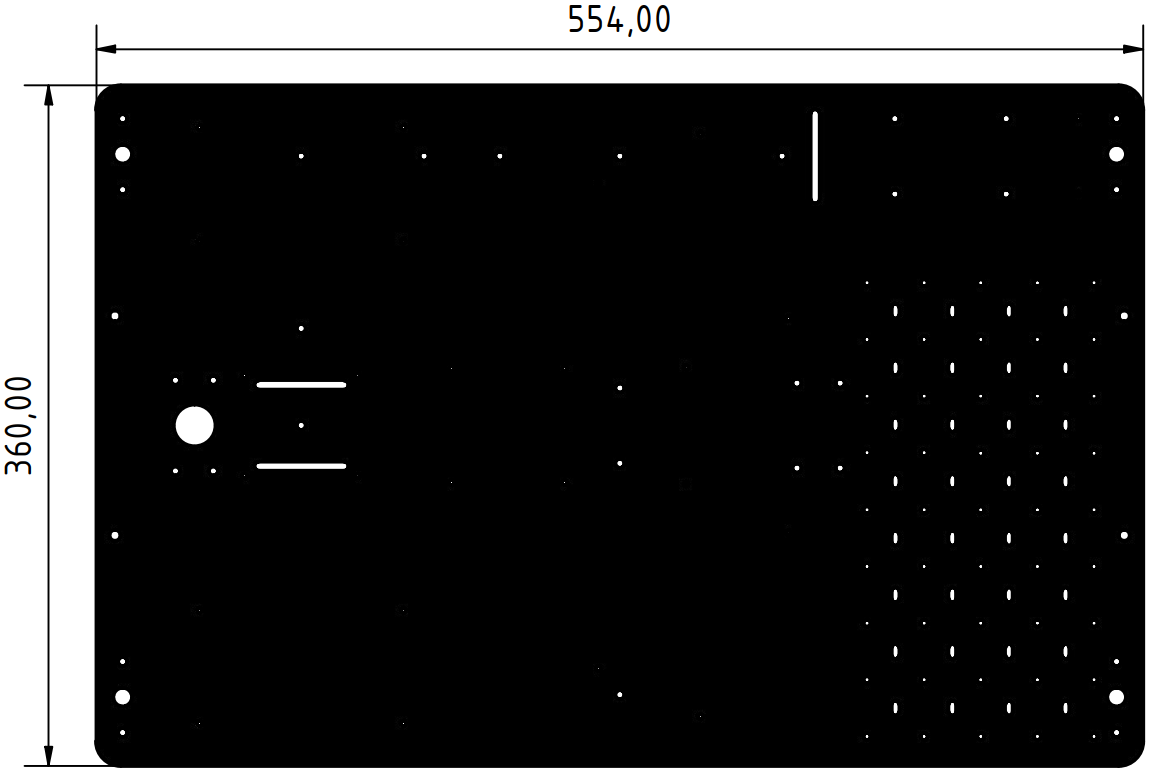
\includegraphics[width=0.95\textwidth]{06disenoConceptual/img/plataforma/baseFijaPlano.png}
    \caption{Plano técnico de la plataforma base con dimensiones finales de 554.00 mm × 360.00 mm. Se muestran los agujeros para insertos roscados M4, agujeros para patas niveladoras M10 en las esquinas, ranuras de cableado y la retícula de montaje en la zona de electrónica. El acabado es negro mate para contraste visual.}
    \label{fig:plataformaBaseVersionFinal}
\end{figure}

Las dimensiones finales de la plataforma son 554 mm de largo por 360 mm de ancho, fabricada en MDF de 9 mm de espesor. Estas dimensiones proporcionan holguras de 6 mm y 3 mm con respecto a las dimensiones internas del contenedor (566 mm × 366 mm), facilitando las operaciones de inserción y extracción de la plataforma.

Todos los elementos geométricos mostrados en el plano (agujeros circulares, ranuras oblongas y el perímetro exterior) son completamente realizables mediante corte láser en una única lámina de MDF. El proceso de corte láser garantiza la precisión dimensional necesaria y permite la fabricación repetible de las 7 plataformas requeridas con tolerancias de ±0.1 mm.

Posterior al corte, cada plataforma se somete al proceso de acabado superficial (lijado, sellado, pintado negro mate y lacado) para garantizar durabilidad y proporcionar el contraste visual necesario para los algoritmos de visión por computador.


\subsection{Componentes Estructurales de la Plataforma Base}

La plataforma base integra diversos componentes estructurales diseñados para proporcionar estabilidad, facilitar el transporte y permitir la gestión ordenada del cableado. A continuación se describen estos componentes y sus especificaciones técnicas.

\subsubsection{Patas Niveladoras}

Las patas niveladoras, mostradas en la Figura \ref{fig:pataNiveladora}, permiten ajustar la horizontalidad de la plataforma para compensar irregularidades en las superficies de trabajo. Cada pata niveladora es un subconjunto compuesto por cuatro elementos:

\begin{figure}[H]
    \centering
    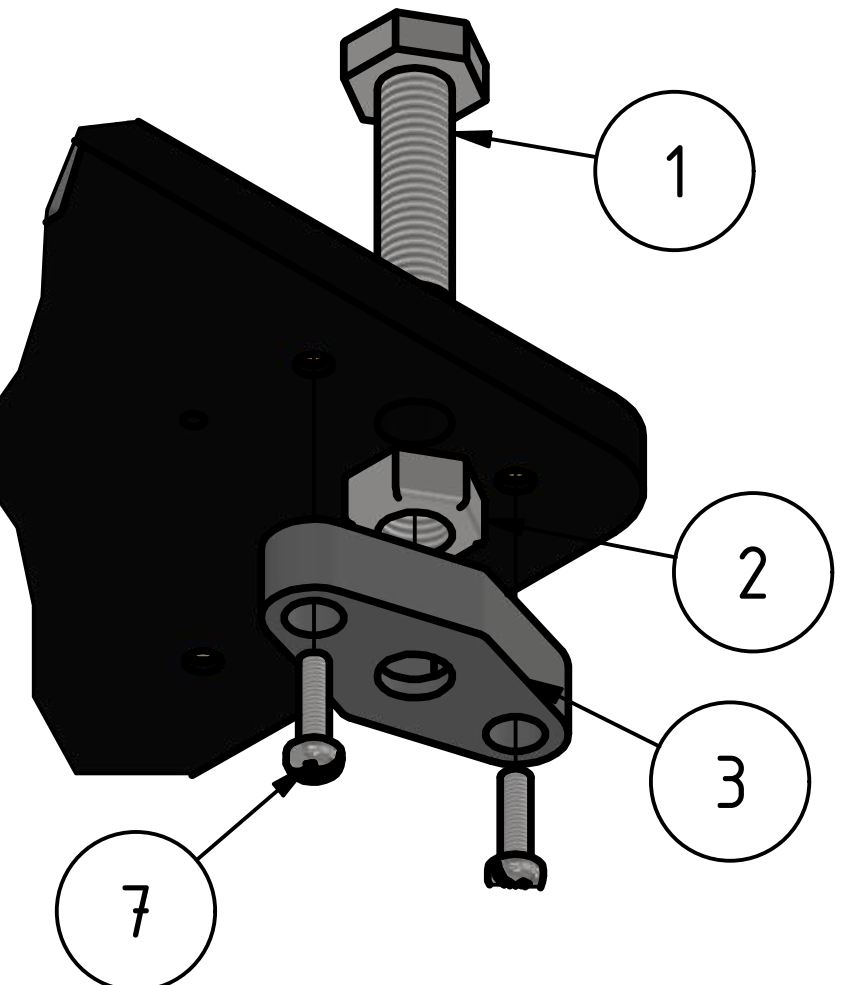
\includegraphics[width=0.5\textwidth]{06disenoConceptual/img/plataforma/pataNiveladora.png}
    \caption{Ensamble de pata niveladora. (1) Tornillo M10 × 35 mm que funciona como elemento de ajuste de altura, (2) Acople impreso en 3D con cavidad hexagonal para alojar la tuerca M10.}
    \label{fig:pataNiveladora}
\end{figure}

\begin{table}[H]
\centering
\caption{Lista de materiales de la pata niveladora}
\label{tab:bom_pata_niveladora}
\small
\begin{tabular}{|c|l|c|l|l|}
\hline
\textbf{\#} & \textbf{Componente} & \textbf{Cant.} & \textbf{Fabricación} & \textbf{Material} \\
\hline
1 & Tornillo M10 × 35 mm & 1 & Comercial & Acero \\
2 & Tuerca M10 & 1 & Comercial & Acero \\
3 & Acople de pata niveladora & 1 & FDM & PLA/ABS \\
4 & Tornillo M4 × 15 mm & 2 & Comercial & Acero \\
\hline
\end{tabular}
\end{table}

El acople de pata niveladora incorpora una cavidad hexagonal que aloja la tuerca M10, impidiendo su rotación. Este acople se fija a la plataforma mediante dos tornillos M4 que se enroscan en insertos roscados ubicados en las esquinas. El tornillo M10 atraviesa la plataforma y el acople, actuando como elemento de ajuste de altura mediante rotación manual.

\subsubsection{Patas de Soporte Central}

Las patas de soporte central (Figura \ref{fig:pataSoporte}) se ubican en la zona media de la plataforma para evitar flexión excesiva cuando se aplican cargas sobre su superficie. Estas patas son especialmente importantes considerando el espesor de 9 mm del MDF y la envergadura de 554 mm de la plataforma.

\begin{figure}[H]
    \centering
    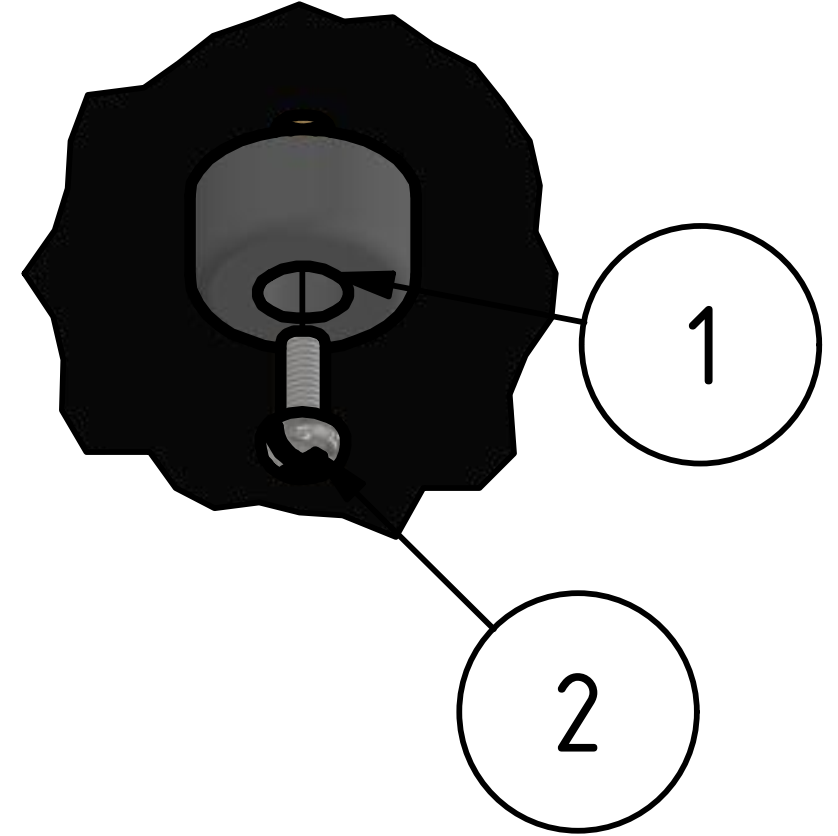
\includegraphics[width=0.45\textwidth]{06disenoConceptual/img/plataforma/pataSoporte.png}
    \caption{Pata de soporte central. (1) Pata fabricada mediante FDM, (2) Vista del montaje en la cara inferior de la plataforma.}
    \label{fig:pataSoporte}
\end{figure}

\begin{table}[H]
\centering
\caption{Lista de materiales de la pata de soporte}
\label{tab:bom_pata_soporte}
\small
\begin{tabular}{|c|l|c|l|l|}
\hline
\textbf{\#} & \textbf{Componente} & \textbf{Cant.} & \textbf{Fabricación} & \textbf{Material} \\
\hline
1 & Pata de soporte & 1 & FDM & ABS/PLA \\
2 & Tornillo M4 × 10 mm & 1 & Comercial & Acero \\
\hline
\end{tabular}
\end{table}

Cada pata se fija mediante un tornillo M4 que se enrosca en un inserto roscado de la plataforma. Se utilizan tres patas de soporte distribuidas en la zona central para proporcionar rigidez estructural sin interferir con las canaletas de cableado.

\subsubsection{Manijas de Transporte}

Las manijas permiten la manipulación ergonómica de la plataforma completa. Su diseño considera datos antropométricos de la población colombiana para garantizar un agarre cómodo y seguro.

\paragraph{Consideraciones Antropométricas}

Según estudios del Imperial College of London y la Asociación Colombiana de Endocrinología, la estatura promedio en Colombia es de 172.4 cm para hombres y 159.3 cm para mujeres. En cuanto a dimensiones de la mano, el ancho de palma es de aproximadamente 8.9 cm para hombres y 7.9 cm para mujeres, mientras que el grosor de los dedos oscila entre 15-20 mm según datos antropométricos internacionales ajustados a la población colombiana. \cite{NCDRisC2020} \cite{Binvignat2012} \cite{Rodriguez2024}

Con base en estos datos, se diseñó una abertura de agarre de 96 mm de ancho. Este valor resulta del compromiso entre comodidad ergonómica (que requeriría anchos mayores) y las restricciones espaciales impuestas por las mangueras neumáticas que conectan la bomba de vacío con el manipulador.

\begin{figure}[H]
    \centering
    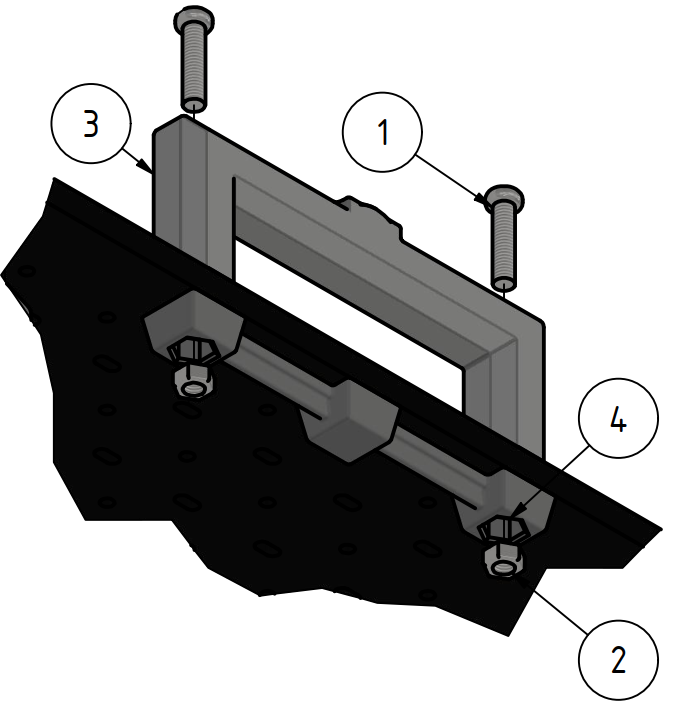
\includegraphics[width=0.6\textwidth]{06disenoConceptual/img/plataforma/manija.png}
    \caption{Ensamble de manija de transporte. (1) Tornillos M6 × 25 mm, (2) Tuercas M6 alojadas en la pata, (3) Cuerpo de la manija (nivel superior), (4) Pata de soporte de la manija (nivel inferior).}
    \label{fig:manija}
\end{figure}

\begin{table}[H]
\centering
\caption{Lista de materiales del subconjunto de manija}
\label{tab:bom_manija}
\small
\begin{tabular}{|c|l|c|l|l|}
\hline
\textbf{\#} & \textbf{Componente} & \textbf{Cant.} & \textbf{Fabricación} & \textbf{Material} \\
\hline
1 & Tornillo M6 × 25 mm & 2 & Comercial & Acero \\
2 & Tuerca M6 & 2 & Comercial & Acero \\
3 & Manija & 1 & FDM & PLA/ABS \\
4 & Pata de manija & 1 & FDM & PLA/ABS \\
\hline
\end{tabular}
\end{table}

El ensamble consta de una manija superior y una pata inferior conectadas mediante dos tornillos M6 que atraviesan completamente la plataforma. Las tuercas M6 se alojan en cavidades de la pata inferior, donde quedan cautivas. La pata cumple una función estructural crítica: proporciona soporte vertical para evitar flexión de la plataforma en caso de que alguien se apoye accidentalmente sobre la manija durante el transporte.

\subsubsection{Sistema de Canaletas}

Las canaletas organizan y protegen el cableado que conecta los diferentes subsistemas del kit. El diseño contempla cuatro canales independientes que permiten el paso de:

\begin{itemize}
    \item Cables de control desde la Raspberry Pi hasta el controlador del manipulador
    \item Cables de alimentación para la bomba de vacío
    \item Manguera neumática de 4 mm de diámetro (configuración actual o futura)
    \item Canal adicional para expansiones futuras
\end{itemize}

\begin{figure}[H]
    \centering
    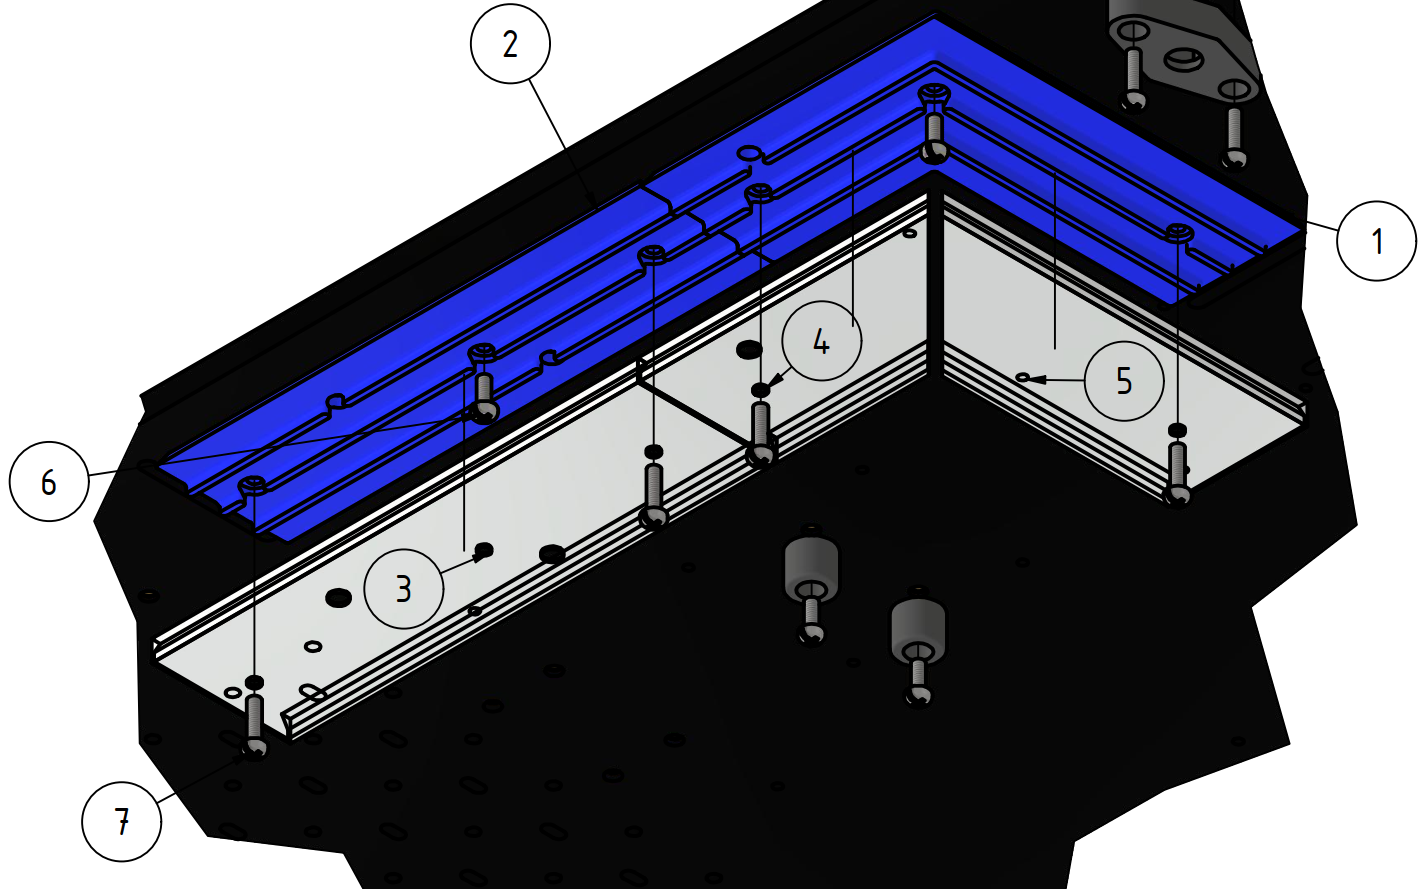
\includegraphics[width=0.8\textwidth]{06disenoConceptual/img/plataforma/canaleta.png}
    \caption{Sistema de canaletas para gestión de cableado. (1) Codo de canaleta, (2) Tapas transparentes en PETG (tres segmentos), (3) Canaleta recta, (4-5) Canales internos para separación de cables, (6) Zona de anclaje con tornillos M4, (7) Tornillos de fijación a insertos roscados de la plataforma.}
    \label{fig:canaleta}
\end{figure}

La canaleta presenta geometría en forma de L, conectando la ranura cercana al controlador con la ranura próxima al manipulador. Debido a las limitaciones del volumen de impresión de las impresoras FDM disponibles, el sistema se divide en dos componentes base:

\begin{itemize}
    \item Codo de canaleta: Sección angular que conecta ambos ejes
    \item Canaleta recta: Segmento longitudinal
\end{itemize}

Las tapas se fabrican en PETG transparente, permitiendo inspección visual del cableado sin necesidad de desmontaje. Esta característica facilita las tareas de mantenimiento y resolución de problemas. La configuración en L de la tapa requiere su división en tres segmentos para viabilizar su fabricación mediante FDM.

\begin{table}[H]
\centering
\caption{Lista de materiales del sistema de canaletas}
\label{tab:bom_canaleta}
\small
\begin{tabular}{|c|l|c|l|l|}
\hline
\textbf{\#} & \textbf{Componente} & \textbf{Cant.} & \textbf{Fabricación} & \textbf{Material} \\
\hline
1 & Codo de canaleta & 1 & FDM & PLA/ABS \\
2 & Canaleta recta & 1 & FDM & PLA/ABS \\
3 & Tapa larga & 1 & FDM & PETG \\
4 & Tapa diagonal 110 mm & 1 & FDM & PETG \\
5 & Tapa diagonal 135 mm & 1 & FDM & PETG \\
6 & Tornillo M4 × 10 mm & 2 & Comercial & Acero \\
7 & Tornillo M4 × 15 mm & 4 & Comercial & Acero \\
\hline
\end{tabular}
\end{table}

El sistema de canaletas se fija a la plataforma mediante tornillos M4 que se enroscan en insertos roscados ubicados estratégicamente en el nivel inferior. Las tapas se deslizan en guías laterales de la canaleta, permitiendo acceso rápido al interior sin necesidad de desmontar completamente el sistema.